In the lecture, the force-length relation of a 1D polymer was calculated
using the microcanonical ensemble.

\paragraph{a) Now do the calculation in the canonical ensemble.
    (\textit{2 points}) \\
    HINT: Consider again a chain of $N$ monomers of size $a$ with $x_i=+a$ or 
    $-a$ and $X=\sum_ix_i$ the total length of the polymer (for the given 
    configuration). Note that the polymer is "ideal", i.e. the distribution of 
    bonds does not change the energy of the chain in the force-free case;
    in turn, under an external force $F$ the energy of this system is given by 
    $E(X)=-FX$.
} \ \\
    \\
    The partition sum for the canonical ensemble is given by 
    \begin{equation}
        Z=\sum_i e^{-\beta E_i}
        \,, \ \ \ \ \ \ \textnormal{with }
        \beta:=\frac{1}{k_BT} \,.
    \end{equation}
    The sum is performed over all configurations $i$ with energy $E_i$.
    Define the length of the polymer as $L = Na$ and the effective length
    of the polymer,
    \begin{equation}
    X=\sum_ix_i=(N_+ - N_-)a=(2N_+ - N)a \,,
	\end{equation}        
    where $N_+$ corresponds
    to the number of monomers with $x_i=+a$ and $N_-$ corresponds
    to the number of monomers with $x_i=-a$. We used the condition $N=N_+ + N_-$. \\
    We need to take into account that there are
    \begin{align}
        \Omega(X)
        =\frac{N!}{N_+! N_-!} = \binom{N}{N_+}
    \end{align}
    different configurations that lead to the same length $X$.
    Thus, the partition sum is given by
    \begin{equation}
        Z=\sum_X\Omega(X) e^{-\beta E(X)}
        =\sum_{i=0}^N \binom{N}{i} e^{-(N - 2i) \beta F a} = \left(e^{\beta F a} + e^{-\beta F a}\right)^N \,.
    \end{equation}
    In the last step, we used the binomial theorem,
    \begin{equation}
        (x+y)^n = \sum_{i=0}^n \binom{n}{i} x^{n-i} y^i \,,
    \end{equation}
    and set $x = e^{-\beta F a}$ and $y = e^{\beta F a}$. 
    Therefore, the partition sum is given by
    \begin{align}
        Z
        &=2^N \cosh\left(\beta Fa\right)^N \\
        &=\bigg(2\cosh\left(\beta Fa\right)\bigg)^N \,.
    \end{align}
    % \begin{equation}
    %     <U>=-\partial_\beta \log Z
    % \end{equation}
    % \begin{equation}
    %     <U>=F<X>
    % \end{equation}

    % Thermodynamical free energy:
    % \begin{equation}
    %     F=k_BT\cdot\log(Z)
    % \end{equation}
    % \begin{itemize}
    %     \item get equations of state
    %     \item differentiate free energy for ?
    %     \item $\Rightarrow$ relationship between force and length $X$
    % \end{itemize}
    % ...
    \noindent
    From the partition sum, we can calculate the system's energy:
    \begin{align}
        \langle E\rangle
        &=-\partial_\beta \ln(Z) \\
        &=-N\cdot\partial_\beta\ln\bigg(2\cosh(\beta Fa)\bigg) \\
        &=-N\cdot\frac{1}{2\cosh(\beta Fa)}\cdot 2\sinh(\beta Fa)\cdot Fa \\
        &=-NFa\cdot\tanh(\beta Fa)
    \end{align}

\newpage
\paragraph{b) Show that your result is identical to the one in the lecture.
    Discuss the limits $Fa<<k_BT$ and $Fa>>k_BT$. (\textit{2 points})
} \ \\
    \\
    Because the system's energy is related to the applied force by 
    $\langle E\rangle=FX$, it follows that 
    \begin{align}
        FX
        &=-NFa\cdot\tanh(\beta Fa) \\
        \Rightarrow X
        &=-Na\cdot\tanh(\beta Fa)
        \label{eq:fx_relation}
    \end{align}
    \textbf{for large $T$:} \\
    Large temperature values lead to a small $\beta$.
    For small input values $x$, we can approximate $\tanh(x)\approx x$.
    Thus, for large temperatures we can rewrite \autoref{eq:fx_relation} as
    \begin{equation}
        F\approx-\frac{X}{Na^2}\cdot k_BT,
    \end{equation}
    which is the result that we already know from the lecture. \\
    % ...
    % \begin{equation}
    %     F\approx-k_BT\cdot\frac{L}{Na^2}
    % \end{equation}
    % \red{(fuer kleine Auslenkungen)}
    \\
    \textbf{for small $T$:} \\
    ... \\
    \\
    \textbf{...} \\
    free energy:
    \begin{align}
        F
        &=-k_BT\cdot\ln(Z) \\
        &=-k_BTN\cdot\ln\bigg(2\cosh(\beta Fa)\bigg) \\
        &=-k_BTN\cdot\ln\bigg(2\cosh\bigg(\frac{Fa}{k_BT}\bigg)\bigg) \\
    \end{align}
    entropy:
    \begin{align}
        S
        &=-\bigg(\frac{\partial F}{\partial T}\bigg)_{V,N} \\
        &=k_BN\cdot\ln\bigg[2\cosh\bigg(\frac{Fa}{k_BT}\bigg)\bigg]
        -k_BTN\cdot\frac{1}{2\cosh\bigg(\frac{Fa}{k_BT}\bigg)}\cdot
        2\sinh\bigg(\frac{Fa}{k_BT}\bigg)\cdot\frac{Fa}{k_BT^2} \\
        % \ln\bigg(2\cosh\bigg(\frac{Fa}{k_BT}\bigg)\bigg) \\
        &=k_BN\cdot\ln\bigg[2\cosh\bigg(\frac{Fa}{k_BT}\bigg)\bigg]
        -\tanh\bigg(\frac{Fa}{k_BT}\bigg)\cdot\frac{NFa}{T} \\
    \end{align}

    \begin{figure}[h!]
        \centering
        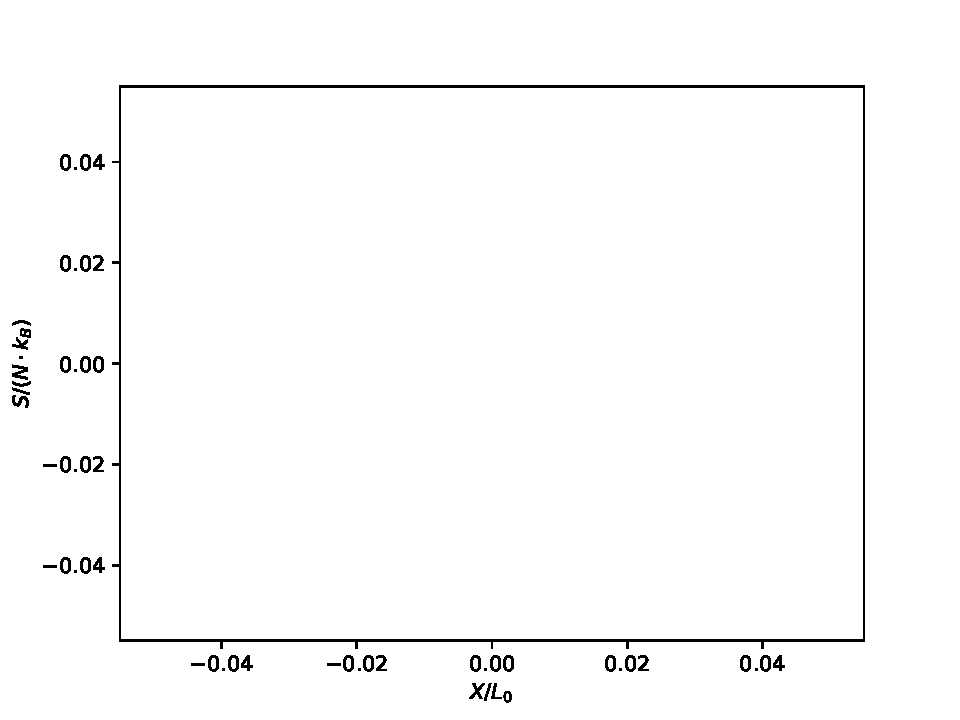
\includegraphics[width=\textwidth]{./figures/entropy.pdf}
    \end{figure} \ \\ 

